\documentclass{article}
% \usepackage[utf8]{inputenc}
\usepackage[pdftex]{graphicx,color}
\usepackage[T1]{fontenc}
\usepackage{lmodern}
\usepackage{amsmath}
\usepackage{amsfonts}
\usepackage{subfigure}
\usepackage{textpos}
\usepackage{verbatim}

% This adds space between the Appendix number (e.g., A.101) and the title.
\renewcommand{\numberline}[1]{#1~}

% If your page numbers stick out into the right-hand margin but using lengths 
% appropriate to your document. See the Introduction to the "The tocloft 
% package" for additional information.
\makeatletter
 \renewcommand{\@pnumwidth}{1.75em} 
 \renewcommand{\@tocrmarg}{3.25em}
\makeatother

% use a larger page size; otherwise, it is difficult to have complete
% code listings and output on a single page
\usepackage{fullpage}

% have an index. we use the imakeidx' replacement of the 'multind' package so
% that we can have an index of all run-time parameters separate from other
% items (if we ever wanted one)
\usepackage{imakeidx}
\makeindex[name=prmindex, title=Index of run-time parameter entries]
\makeindex[name=prmindexfull, title=Index of run-time parameters with section names]

% be able to use \note environments with a box around the text
\usepackage{fancybox}
\newcommand{\note}[1]{
{\parindent0pt
  \begin{center}
    \shadowbox{
      \begin{minipage}[c]{0.9\linewidth}
        \textbf{Note:} #1
      \end{minipage}
    }
  \end{center}
}}

% use the listings package for code snippets. define keywords for prm files
% and for gnuplot. You may want to adapt this for other types of input files or postprocessing scripts. 
\usepackage{listings}
\lstset{
  language=C++,
  showstringspaces=false,
  basicstyle=\small\ttfamily,
  columns=fullflexible,
  keepspaces=true,
  frame=single,
  breaklines=true,
  postbreak=\raisebox{0ex}[0ex][0ex]{\hspace{5em}\ensuremath{\color{red}\hookrightarrow\space}}
}
\lstdefinelanguage{prmfile}{morekeywords={set,subsection,end},
                            morecomment=[l]{\#},escapeinside={\%\%}{\%},}
\lstdefinelanguage{gnuplot}{morekeywords={plot,using,title,with,set,replot},
                            morecomment=[l]{\#},}


% use the hyperref package; set the base for relative links to
% the top-level aspect directory so that we can link to
% files in the aspect tree without having to specify the
% location relative to the directory where the pdf actually
% resides
\usepackage[colorlinks,linkcolor=blue,urlcolor=blue,citecolor=blue,destlabel=true,baseurl=../]{hyperref}

\newcommand{\manual}{\textsc{Software Manual Template}}

\begin{document}

%%%%%%%%%%%%%%%%%%%%%%%%%%%%%%
%%% START OF CIG MANUAL COVER TEMPLATE %%%
%%%%%%%%%%%%%%%%%%%%%%%%%%%%%%
% This should be pasted at the start of manuals and appropriate strings entered at locations indicated with FILL.
% Be sure the TeX file includes the following packages.
% \usepackage{graphicx}
% \usepackage{times}
% \usepackage{textpos}

\definecolor{dark_grey}{gray}{0.3}
\definecolor{aspect_blue}{rgb}{0.3125,0.6875,0.9375}

%LINE 1%
{
\renewcommand{\familydefault}{\sfdefault}

\pagenumbering{gobble}
\begin{center}
\resizebox{\textwidth}{!}{\textcolor{dark_grey}{\fontfamily{\sfdefault}\selectfont
COMPUTATIONAL INFRASTRUCTURE FOR GEODYNAMICS (CIG)
}}

\hrule

%LINE 2%
\color{dark_grey}
\rule{\textwidth}{2pt}

%LINE 3%
\color{dark_grey}
% FILL: additional organizations
% e.g.: {\Large Organization 1\\Organization 2}
{\Large }
\end{center}

%COLOR AND CODENAME BLOCK%
\begin{center}
\resizebox{\textwidth}{!}{\colorbox
% FILL: color of code name text box
% e.g. blue
{aspect_blue}{\fontfamily{\rmdefault}\selectfont \textcolor{white} {
% FILL: name of the code
% You may want to add \hspace to both sides of the codename to better center it, such as:
% \newcommand{\codename}{\hspace{0.1in}CodeName\hspace{0.1in}}
\hspace{0.1in}\manual{}\hspace{0.1in}} }}
\\[12pt]
{\Large LaTeX Template for CIG Software User Manuals}
\end{center}

%MAIN PICTURE%
\begin{textblock*}{0in}(1.5in,0.3in)
% FILL: image height
% e.g. height=6.5in
\begin{center}
\vspace{1em}
\includegraphics[height=3.5in]
% FILL: image file name of your software
% e.g. cover_image.png
{cover_image.png}
\hspace{5em}
\end{center}
\end{textblock*}

%USER MANUAL%
\color{dark_grey}
\hfill{\Huge \fontfamily{\sfdefault}\selectfont Example User Manual \\
\raggedleft \huge \fontfamily{\sfdefault}\selectfont Version
% keep the following line as is so that we can replace this using a script:
0.1.0-pre %VERSION-INFO%
\\\large(generated \today)\\
{\Large Lorraine Hwang\\John Naliboff\\Juliane Dannberg\\Rene Gassm{\"o}ller\\Louise Kellogg\\Hiro Matsui\\}
}


%AUTHOR(S) & WEBSITE%
\null
\vspace{17em}
\color{dark_grey}
{\fontfamily{\sfdefault}\selectfont
% FILL: author list
% e.g. Author One\\Author Two\\Author Three\\
% be sure to have a newline (\\) after the final author
\large
\noindent with contributions by: \\
    John Doe,
    Jane Doe\\
\vspace{1.0em}

{\noindent
{\href{https://geodynamics.org}{geodynamics.org}}
}
}


%LINE%
{\noindent
\color{dark_grey}
\rule{\textwidth}{2pt}
}

%COPYRIGHT STATEMENT
\textcopyright Copyright 2018, Regents of the University of California

}

\pagebreak
\pagenumbering{arabic}

%%%%%%%%%%%%%%%%%%%%%%%%%%%%%%
%%%   END OF CIG MANUAL COVER TEMPLATE    %%%
%%%%%%%%%%%%%%%%%%%%%%%%%%%%%%

\tableofcontents
\pagebreak

% To automatically generate an itemized list of tables and figures, use the commands (commented out) below
% \listoffigures
% \pagebreak
% \listoftables
% \pagebreak

\note{\textbf{Some guidelines on formatting the cover.}

The cover usually includes:
\begin{itemize}
\item The name of the software (just replace the text \textsc{Software Manual Template} in the blue box). 
\item Spiffy cover picture, typically an example of a computational model generated by the program.
\item Version number. 
\item A list of authors and contributors. 
\item Copyright statement. 
\end{itemize}
}

\section{Introduction}

This document provides some guidelines on how to write a software manual for CIG community codes. This includes advice on what content to include and how to format the document using LaTeX. The exact section headings, numbering, and order of presentation may depend on the specific software package. 
If you use the commands provided in this template, LaTeX will handle the numbering of sections, figures, and tables for you and automatically generate a table of contents and list of references. 

\note{You can always include short notes, tips, hints and warnings by using shadowboxes. Insert them using the \texttt{\textbackslash note\{\}} command.} 

Start with an introduction that provides the information you want your users to be aware of when they start using your software. 
In particular, include the history of the code and any points you wish to emphasize as outlined in the following sections. 

\subsection{Overview} Include an overview of your software package, its features, the problem it is designed to solve (including example applications), and (optionally) its development history. In addition, you may want to add other points that are important to you like development principles, words of encouragement soliciting feedback and contributions from the community, or just a link to the official website or mailing list. 

\subsection{Referencing your software.} How to cite the code, relevant scientific publications and the manual (if applicable). You can also link to an external page if you want to have your citation information in only one place (which will make it easier to update). 

\paragraph{Example:} 
When referencing \textsc{softwareName} please cite the following
\cite{softwareName-doi-v1.0.0}
\cite{softwareNamemanual}
\cite{ScientificPaper}
:


{\tt 
\begin{lstlisting}[frame=single,language=ksh]
@misc{softwarename-doi-v1.0.0,
  title        = {{softwareName} v1.0.0 [software]}, 
  author       = {Jill Tumble and
                  Jack Crown and others},                  
  month        = August, 
  year         = 2018,
  DOI          = {myDOI}, 
  URL          = {https://doi.org/myDOI},
  organization = {Computational Infrastructure for Geodynamics}, 
  address      = {Davis, CA}, 
}

@article{softwareNamemanual
  title         = {{\textsc{softwareName}: My User Manual}},
  author        = {Jill Tumble and
                   Jack Crown and others},                
  year          = {2018},
  month         = {August},
  DOI           = {myDOI},
  note          = {doi: myDOI},
  URL           = {https://doi.org/myDOI}
}

@article{ScientificPaper,
  title         = {New scientific models using {\textsc{softwareName}}},
  author        = {Jill Tumble and 
                   Jack Crown and others},                
  year          = {2018},
  journal       = {Journal of Important Scientific Research},
  volume        = {3.14159},
  pages	        = {2.71828},
  DOI           = {myDOI},
  note          = {doi: myDOI},
  URL           = {https://doi.org/myDOI}
}
\end{lstlisting}
}

\note{See also \url{https://geodynamics.org/cig/abc} for more information on how to cite software.}

\subsection{Support} 
Acknowledge sources of support including grants, fellowships, etc.
In particular, please acknowledge CIG as follows:
{\parindent0pt
  \begin{center}
    \shadowbox{
      \begin{minipage}[c]{0.9\linewidth}
\textsc{softwareName} is hosted by the Computational Infrastructure for Geodynamics (CIG)
which is supported by the National Science Foundation award EAR-1550901.
      \end{minipage}
    }
  \end{center}
}

\subsection{Disclaimers} State any warranties and disclaimers (if applicable).

\section{Methods/Theoretical Background}

You probably want to provide some background on the methods used in your software. Even if they are available as a separate publication, it is worth it to reference relevant publications and provide a short summary here. 
This section would typically include points like:

\begin{itemize}
\item Governing equations. Describe the physics of the model implemented. Include boundary conditions, definition of coefficients, and approximations. Include other conditions if applicable.
\item Computational approach. Describe the numerical methods used.
\item Reference frame and coordinate systems.
\item Naming conventions.
\item Units. Are the units mks, cgs, non-dimensional?
\item Features. Add sections on additional features as necessary.

\end{itemize}

\section{Installation}

It is very important to provide detailed instructions on how to install your software. Your users may want to run it on different platforms, and if your software depends on other libraries and/or the installation process is complicated, this may be a barrier for potential users. 
Hence, make sure to include:
\begin{itemize}
\item Software and hardware requirements.
\item Instructions on configuring and compiling the source code. Describe how to install your software locally. Include software requirements and special instructions for different platforms and compiling options.
If you include specific instructions, for example on how to install the software using the command line, highlight them by using the lstlisting environment provided by the \texttt{listing} package:
\begin{lstlisting}[frame=single,language=ksh]
git clone YourGitRepository/YourPackageName
mkdir build; cd build; cmake ..
make
\end{lstlisting}

\item Alternative installation instructions. It may take beginners some time to install your software on their local system, so you may want to include some simple alternative such as availability as binaries, virtual machines, and/or containers.

\textbf{Example.}
\begin{lstlisting}[frame=single,language=ksh]
docker pull YourDockerRepository/YourPackageName
\end{lstlisting}

\item If your software runs in parallel, you may want to provide instructions or scripts for installing it on a supercomputer. This can be very helpful, particularly if you (or other users/developers) have experience with specific supercomputers your community may want to use. 
\item High level outline of software components (if applicable).
\item Example Test. A simple test case(s) that allows the users to make sure the program is installed correctly and can be run.
\item Support. How to get help with installing your software.
\end{itemize}

You can also include a table that provides an overview over the differnt installation options (see Table~\ref{tab:install-options}). 

\begin{table}[htb]
  \center
  \begin{tabular}{|c|ccc|}
    \hline
    Feature & Compile \& Install & Virtual Machine & Docker Container \\
    \hline
    Disk overhead           & 0~GB  & 1~GB        & 200~MB \\
    Knowledge required      & Much  & Very Little & Little \\
    MacOS support           & Yes   & Yes         & Yes    \\
    Windows support         & No    & Yes         & Yes    \\
    ...                     & ...   & ...         & ... \\ \hline
  \end{tabular}
  \caption{Example table. Features of the different installation options of your software.}
  \label{tab:install-options}
\end{table}

\section{Getting Started}

Now that the users know how to install your software, you want to teach them how to run it. If you have tutorials online, you can provide links here. 
Some useful points are provided in the following subsections. 

\subsection{Running the code and workflow} 
Provide a simple overview of the entire workflow with example input files of how to run the code (quick start).
A good overview should include a workflow diagram. Include the steps necessary to create program inputs and post-processing outputs if necessary.

\subsection{Inputs} 
Describe structure of input files (if applicable) and runtime options.
If you have a lot of options, it might be worth it to list them in the appendix, and only outline some general options and examples here. 

\subsection{Outputs} Describe the generated output files and how to use them, showing simple examples. Once users have setup and run their first numerical model using your software, they will want to know how to analyze and look at the models results. Hence, make sure to include:
\begin{itemize}
\item Advice of how to visualize the output. Describe necessary steps and tools to look at the results, for example using Paraview, VisIt, Python or gnuplot. 
\item Post-processing. Describe and provide examples of common post-processing operations, and include example scripts if applicable.
\end{itemize}

These instructions are particularly useful if you include images that show what you are describing (see Figure~\ref{fig:paraview}).

\begin{figure}[tbp]
  \centering
  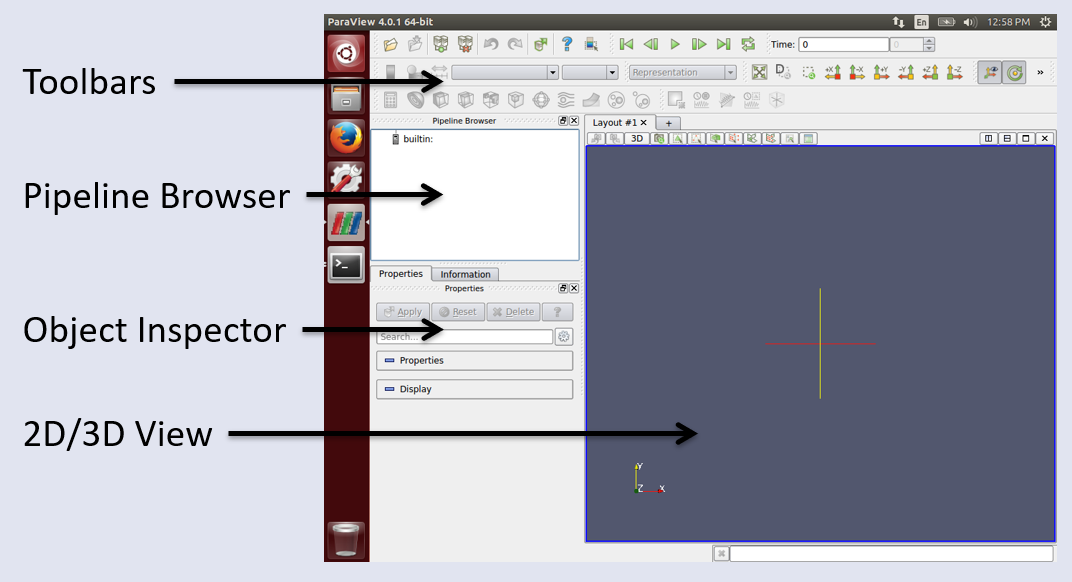
\includegraphics[width=0.6\textwidth]{paraview.png}
  \caption{\it Example of a figure. Make sure to add some figures that show how to visualize model results.}
  \label{fig:paraview}
\end{figure}

\section{Benchmarks, Cookbooks, Examples}

Now that users know how to run the code and how to write input files, 
they may want to set up a model corresponding to their research interests. 
To make that easier for them, it can be helpful to provide a number of example models, starting from very simple setups and becoming more and more complex step by step. It can even be worth it to include some examples from publications that have used your software as final examples, so that the users also learn how they can setup complex models. 
Three specific types of examples are:

\begin{itemize}
\item Simple setups. These examples teach how to use one specific feature of the code, but are otherwise very simple. This can include examples for pre- and/or post processing.
\item More realistic examples/applications. These more complex models could be applications of your code to a specific geophysical problem or setup, and users can adapt for their own research use..
\item Benchmarks. Include examples of benchmarks used to demonstrate that the code (or a specific feature of it) is working correctly.
\end{itemize}

In general, you want to make sure that you explain both the specific feature or physical mechanism you want to showcase in your respective example, and how to set up this feature in the input file options. 

\section{Troubleshooting}

Often, there are specific problems that many users run into, or frequently asked questions. So make sure that your users know how to find solutions or where to find help!

Common points are:
\begin{itemize}
\item Troubleshooting. How to troubleshoot common errors.
\item Resources. Where to look for for help. Can also include supplemental materials e.g. links to tutorials or a website.
\item Mailing lists. Appropriate mailing lists to connect with the community and get help.
\item Bugs and Issues. If users find a bug or spot a problem, make sure that they will let you know! (One option could be explaining how to open an issue on  platform like github, but you may have other policies.)
\end{itemize}

\section{Contributing}

This section should contain a guide for how to contribute to your project. It should describe both the technical procedure of proposing changes to your software, and some guidelines on what type of features you would like users to contribute in which way. 
It is always some additional effort to contribute code to the main repository, so make sure that users have some motivation for doing it and that it is as easy as possible for them. We suggest to make it clear that your software is a welcoming community project to lower the barrier that keeps new users from contributing. 

\section{Acknowledgements}
Remember to acknowledge other contributors and/or software packages and libraries used as appropriate.

\appendix
\pagebreak

% print the list of references. make sure the page number in the index is
% correct by putting the \addcontentsline inside the command that prints the
% title of the page, see http://www.dfki.de/~loeckelt/latexbib.html
% see manual.bib for references
\let\myRefname\refname
\renewcommand\refname{%
  \addcontentsline{toc}{section}{\numberline{}References}
  \myRefname
}
\bibliographystyle{abbrvurl}
\bibliography{manual}

\pagebreak
\section {Appendices}
\begin{itemize}
\item Parameters. Definition of parameters
\item License. A full copy of the license
\item Glossary. Definition of specialized terms
\item File formats. Description of software specific file formats and specifications

\end{itemize}

\end{document}
